\subsection{Analyse der Ergebnisse} \label{analyse-subsec}


Es sei darauf hingewiesen, dass L{\"o}sungen, die auf der Verwendung von Deep Neural Networks (DNNs) zur Extraktion von Merkmalen basieren (z.B. Multi-Layer-Perceptron, Convolutional Neural oder Long-Short-Term-Memory Networks) ebenfalls getestet wurden. Diese Ans{\"a}tze konnten aber nicht so gute Ergebnisse erzielen, wie die handgefertigten Merkmale. Erkennungsraten f{\"u}r die am wenigsten vertretenen Klassen (insbesondere ``Frustration'') scheinen der Grund f{\"u}r die schwache Performance der DNNs zu sein. Wir gehen davon aus, dass dieses Ph{\"a}nomen durch die relativ geringe Gr{\"o}{\ss}e unseres Datensatzes verursacht wird. \\

Entgegen unserern Erwartungen liefert der CA sch{\"a}chere Performance als die handgefertigten Merkmale. Der Grund hierf{\"u}r ist aber sehr wahrscheinlich der selbe wie bei den  DNNs, und zwar der relativ kleine Datensatz. 
Eine kleine qualitative Analyse der in der Studie verwendeten Daten kann die Gr{\"u}nde f{\"u}r diese Beobachtungen begr{\"u}nden. 
CA-Merkmale (sowohl f{\"u}r weiche als auch f{\"u}r harte Zuweisungen) sind per Definition sehr empfindlich gegen{\"u}ber Variationen der Formen der Originalsignale: Die Codew{\"o}rter werden durch Clustering auf S{\"a}tzen von Segmenten bestimmt, die aus den Originalsignalen extrahiert wurden, und die histogrammbasierten Merkmale selbst basieren auf direkten Vergleichen zwischen den Codew{\"o}rtern und dem Segment der zu klassifizierenden Daten. 
Daher kann jede Quelle von Rauschen oder Unregelm{\"a}{\ss}igkeiten in den Originaldaten die Effektivit{\"a}t der CA-Funktionen stark beeintr{\"a}chtigen. 
Ein Blick auf die in unserer Studie verwendeten Signale ergab zwei Hauptprobleme: falsche Datenwerte, die durch Hardwareprobleme bei einigen Sensoren verursacht wurden (wie in Abbildung \ref{fig:bad_signals}), und das Vorhandensein von Rauschen, das Unregelm{\"a}{\ss}igkeiten in den Signalformen verursacht (siehe Abbildung \ref{fig:zoom}). M{\"o}gliche L{\"o}sungen zur Behebung dieses Problems k{\"o}nnten sein, zus{\"a}tzliche Vorverarbeitungstechniken zur Rauschunterdr{\"u}ckung einzusetzen, wie z.B. Tiefpassfilterung. \\


\begin{figure}[h]
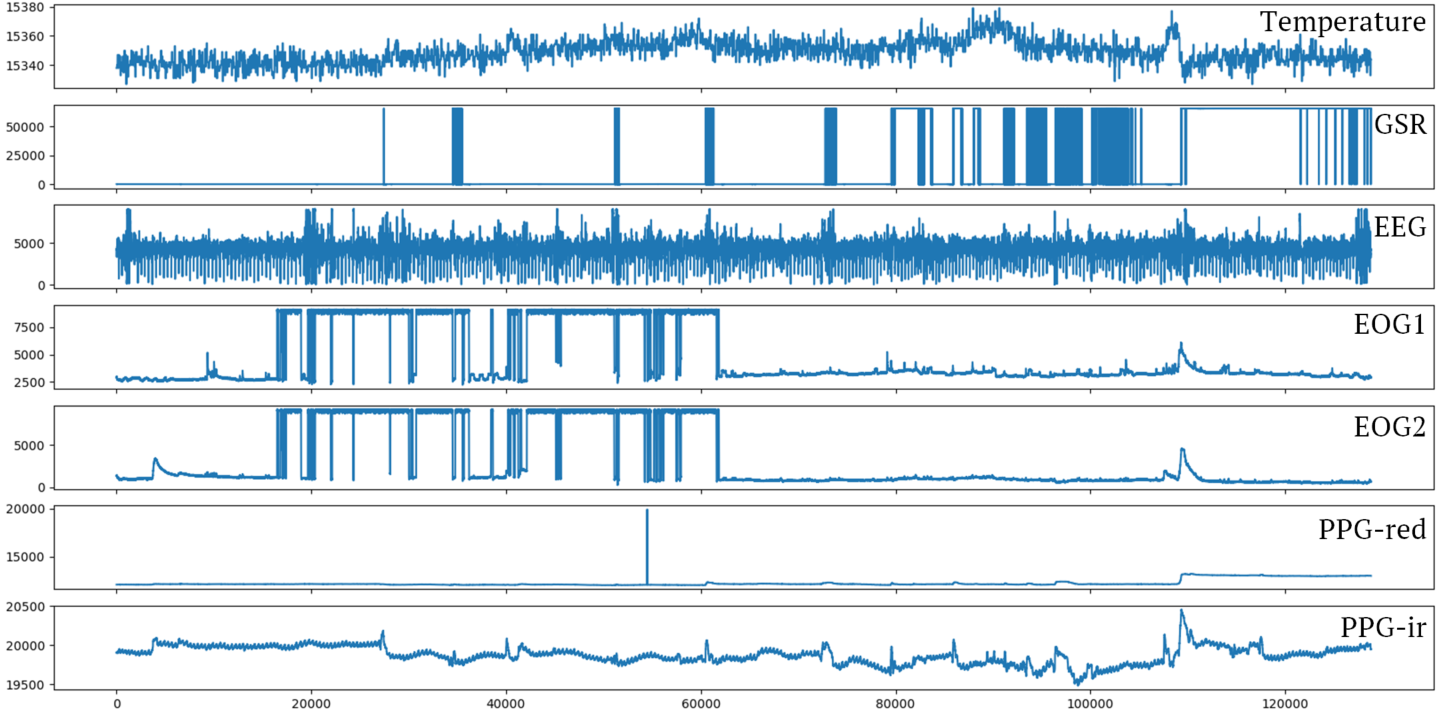
\includegraphics[width=\textwidth]{Images/bad_signals.png} 
\vspace{-0.3cm} \caption[Sensoraufzeichnungen von Daten]{ Sensoraufzeichnungen von Daten, die im Rahmen des ELISE-Projekts von einem der drei getesteten Probanden erfasst wurden. Die x-Achse repr{\"a}sentiert die Zeit und die y-Achse die Sensorwerte. Die in den Daten von GSR und den beiden EOG-Kan{\"a}len sichtbaren Unregelm{\"a}{\ss}igkeiten deuten auf Probleme mit der Hardware hin. }
\label{fig:bad_signals} \end{figure} \vspace{0.5cm}


\begin{figure}[h]
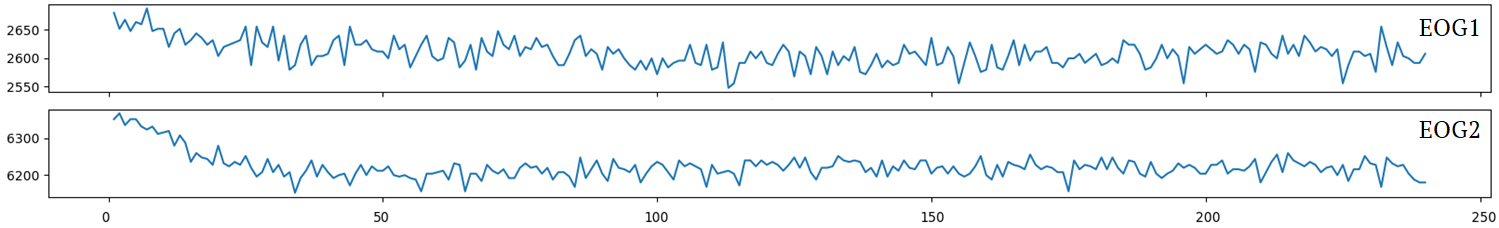
\includegraphics[width=\textwidth]{Images/zoom.png} 
\vspace{-0.3cm} \caption[Nahaufnahme von Rauschen in Daten]{ Nahaufnahme der im Rahmen des ELISE-Projekts erworbenen EOG-Kan{\"a}le von einem der drei getesteten Probanden. Das Vorhandensein von Rauschen in den Daten ist sichtbar, das zu Unregelm{\"a}{\ss}igkeiten in den Signalformen f{\"u}hrt. }
\label{fig:zoom} \end{figure} \vspace{0.5cm}



\newpage

Allgemein deuten die Ergebnisse aber darauf hin, dass unser biomedizinisches Datenerfassungssystem zur Emotionserkennung erfolgreich eingesetzt werden k{\"o}nnte, um ein intelligent adaptives Lernsystems zu verbessern. Zuk{\"u}nftige Arbeiten werden die Verfeinerung des Multisensor-Datenerfassungsger{\"a}tes, die Erfassung weiterer und gr{\"o}{\ss}erer Datens{\"a}tze f{\"u}r die weitere Mustererkennungsanalyse und die Analyse der Wirksamkeit des Emotionserkennungssystems in einem VR-affektiven Lernkontext beinhalten.